\chapter{2013年财务报告}
\section{2013年度财务工作报告}

\indent
2013全年生产滤棒161.27亿支,销售162.36亿支,实现利税总额6877万元,其中:实现利润总额4869万元、实现税金合计3302 万元,圆满完成2013年度经营目标。现将2013年度的财务状况及资产运营情况分析汇报如下:

一、资产营运效率

2013年总资产周转次数为2.14次,比上年同期周转次数增加0.06次;流动资产周转率比上年增加0.06次,与上年基本持平。

二、营运能力

存货周转8.3次、应收帐款周转6.9次,分别比上年同期增加0.17次、下降0.4次,公司营运能力和上年基本持平。


三、偿债能力

流动比率7.14次,同比增加1.32点,主要原因为期末存货的比重下降,速动比率4.8次,同比提高1.24点,与国际标准值2和1相比,有所增加,公司偿还短期债务的风险进一步提高;因合并报表要求,应付川渝公司货款全额冲抵,影响资产负债率由上年9.82\%,下降到9.12\%、下降0.7\%资产负债率偏低。公司无长期负债。从资产负债率和产权比率来看,公司的资本结构稳健,说明股东的投资风险低。


四、盈利能力

    2013年销售毛利率为13.9\%,销售净利率为5.6\%,成本费用利润率为8.53\%,净资产收益率为13.26\%,分别比去年下降0.76\%、0.53\%、0.54\%、2.08\%;盈利能力转弱的主要原因为消化可光降解丝束价格成本、新增固定资产投资的折旧增加、人工、制造成本、搬运费、运输费、仓储费等刚性增加。


五、期间费用情况:

公司根据生产经营实际需要,严格遵守中央“八项规定”和“九条要求”,严格控制重点费用支出,受刚性增长因素影响,部分费用较2012年有所增加,但未超过年度预算目标。管理费用总额较2012年增加208万元,营业费用较2012年增加13万元。其中:工资增加46万元、折旧增加72万元、审计咨询费增加6万元、库房租赁增加20万元、运输费增加26万元、技术研发费增加80万元、修理费增加4万元、警卫消防费增加12万元、车辆费用增加10万元、涉外费用增加11万元、坏账准备增加41万元。
重点费用中:
业务招待费实际执行110万元,同比下降43万元、28\%;会议费因严格执行中央“八项规定”、国家局“九条要求”,年度内未组织召开会议,费用同比下降16万元,下降99\%;宣传业务促销因招投标时间延迟原因,年度实施2.24万元,完成预算的3.68\%;涉外费用实际执行26万元,因培训人员增加,同比增加11万元,增加73\%。

\subsection{2013年度资产负债情况}
见附录~\ref{app:appendix1-1}

\subsection{2013年度利润分配情况}
见附录~\ref{app:appendix1-2}

\subsection{2013年度财务状况和经营成果情况}

{\dawuhao \song {  %此处写字体大小控制命令
\begin{center}
  \renewcommand{\arraystretch}{1.4}
\begin{longtable}{|p{0.25\textwidth}<{\centering}|p{0.15\textwidth}|p{0.15\textwidth}|p{0.15\textwidth}|p{0.1\textwidth}|}
    \caption{2013年度财务状况和经营成果情况表}\\
  \spacecell{} & \spacecell{} & \spacecell{} & \spacecell{} & \spacecell{{单位:万元}}\\
\hline
\hline
\rowcolor{darkblue!20}
 \sf 项目  & \sf 2012年度 & \sf 2013年度 &
 \sf 增减 & \sf  增幅  \\
\hline
\endfirsthead    % endfirsthead      %%%需要定义两个头两个尾的样式
%
\multicolumn{5}{c}{\bf{2013年度财务状况和经营成果情况表(续表)}}\\
\hline
\rowcolor{lightblue}
项目   &  \sf 2012年度 & \sf 2013年度 & \sf 增减 & \sf 增幅 \rule{0pt}{20pt} \\
\hline
\endhead         % endhead
%
%%%%
\hline
\multicolumn{5}{r}{\emph{ 续下页 \ldots}}
\endfoot          % endfistfoot
%
\hline
\endlastfoot       % endfoot
  \hline
主营业务收入&58162&62091&3929&6.75\%\\
  \hline
主营业务成本&49638&53463&3825&7.7\%\\
  \hline
销售税金&229&193&-36&-15.7\%\\
  \hline
经营费用&601&614&13&2.1\%\\
  \hline
管理费用&2779&2987&208&7.48\%\\
  \hline
财务费用&-7&-6&1&14.2\%\\
  \hline
其他业务利润&28&28&&\\
  \hline
营业外收入&28&7&-21&-75\%\\
  \hline
营业外支出&53&6&-47&-88.6\%\\
  \hline
利润总额&4836&4869&33&0.68\%\\
  \hline
 \multicolumn{1}{|>{\columncolor{mycyan}\sf }l|}{ 资产营运状况:}&&&&\\
  \hline
总资产周转率&2.08&2.14&0.06&2.9\%\\
  \hline
流动资产周转率&3.34&3.4&0.06&1.8\%\\
  \hline
存货周转&8.13&8.3&0.17&2.1\%\\
  \hline
应收账款周转&7.3&6.9&-0.4&-5.47\%\\
  \hline
资产损失比率&0&0&&\\
  \hline
 \multicolumn{1}{|>{\columncolor{mycyan}\sf }l|}{ 偿债能力状况:}&&&&\\
  \hline
流动比率&5.82&7.14&1.32&22.68\%\\
  \hline
速动比率&3.56&4.8&1.24&34.8\%\\
  \hline
资产负债率&9.82\%&9.12\%&-0.7&-7.1\%\\
  \hline
产权比率&10.85&10.04&-0.81&-7.46\%\\
  \hline
 \multicolumn{1}{|>{\columncolor{mycyan}\sf }l|}{ 财务效益状况:}&&&&\\
  \hline
销售毛利率&14.66\%&13.9\%&-0.76\%&-5.18\%\\
  \hline
成本费用利润率&9.07\%&8.53\%&-0.54\%&-6\%\\
  \hline
销售净利率&6.13\%&5.6\%&-0.53\%&-8.6\%\\
  \hline
净资产收益率&15.34\%&13.26\%&-2.08\%&-13.56\%\\
  \hline
总资产利润率&17.34\%&16.38\%&-0.97&-5.59\%\\
  \hline
资本保值增值率&116.62\%&114.16\%&-0.97&-5.59\%\\
  \hline
 \multicolumn{1}{|>{\columncolor{mycyan}\sf }l|}{ 发展能力:}&&&& \\
  \hline
销售增长率&8.72\%& 6.78 \%&-1.94&-22\%\\
  \hline
资本积累率&16.62\%&14.16\%&-2.46&-14.8\%\\
  \hline
总资产增长率&-0.66\%&13.32\%&13.98&\\
  \hline
固定资产成新率&49.42\%&    52\%&2.58&5.2\%\\
  \hline
\end{longtable}
\end{center}
}}

%%%%%%%%%%%%%%%%%%%%%%%%%%%%%%%%%%%%%%%%%%%%%%%%%%%%%%%%%%%%%%%%%%%%%%%%%%%%%%%%%%%%%%%555


\section{2013年度财务预算执行情况报告}

2013年我们围绕公司生产经营目标,继续强化预算的刚性管控,严格遵照执行川渝公司对重点费用预算的控制要求,通过报帐中心平台,发挥预算管理监控职能,做到预算适时监督、及时、准确反映各部门预算执行进度和存在问题的原因,强化了预算执行情况分析和考核。通过班子和各部门的共同努力,全员全面预算管理意识进一步得到强化,2013年各主要预算项目完成进度正常,费用预算控制在预算进度目标内;资本性投资支出严格按程序立项申报实施。具体分析如下:

\subsection{总体情况}

%%%%%%%%%%%%%%%%%%%%%%%%%%%%%%%%%%%
\vspace{1cm}
\begin{table}[!htbp]
      \renewcommand{\arraystretch}{1.2}
%  \arrayrulewidth                     %%% 定义\hline, \vline,\cline及列定义的分隔线|的线宽
%  \addtolength\doublerulesep{4pt}      %%% 定义连续两个\hline或两个|所画的线段之间的间隔
 \centering
    \caption{2013年主要预算指标执行情况表}
 \begin{tabular}
   {|>{\sf}p{0.34\textwidth}|p{0.18\textwidth}<{\centering}|p{0.18\textwidth}<{\centering}|p{0.15\textwidth}<{\centering}|}
   \spacecell{}& \spacecell{}& \spacecell{}&\spacecell{{\sihao 单位:万元}}\\
  \hline
%  \rowcolor{mycyan}
  & \sf 2013年实际 & \sf 年度预算 & \sf    执行进度\\
  \hline \hline
  \multicolumn{1}{|>{\columncolor{mycyan}\sf}l|}{一、税利合计} & 6877&	6022.08	&114.2\%  \\
  \hline
  \multicolumn{1}{|>{\columncolor{mycyan}\sf}l|}{二、应交税金合计} & & & \\
  \hline
 \hfill 其中:应交增值税 & 1772&	935.31	& 189.45\%  \\
  \hline
\hfill 应交消费税 & & &\\
  \hline
 \multicolumn{1}{|>{\columncolor{mycyan}\sf }l|}{ 三、利润总额} & 4869.05&4919.09&98.99\%  \\
  \hline
 \hfill 其中:主营业务收入 & 62090.9&56932.5&109.06\%  \\
  \hline
 \hfill 主营业务成本 & 53462.65&47984.44&111.42\%  \\
  \hline
 \hfill 销售税金及附加 & 193.40&111.93&172.79\%  \\
  \hline
\hfill 期间费用 & 1508.60&1967.78&76.67\%  \\
  \hline
\hfill 营业外收支净额 & -24.78 & 75 & -33.1\%  \\
  \hline
\end{tabular}
 \end{table}


\newpage
  \subsection{产销情况}

\begin{table}[!htbp]
    \renewcommand{\arraystretch}{1.3}
 \centering  \caption{2013年产销情况表}
% \hfill 单位:万支\quad
 \begin{tabular}{@{}>{\hei}ccccccc@{}}
  \spacecell{} & \spacecell{} & \spacecell{} &   \spacecell{} & \spacecell{} & \spacecell{} &  \spacecell{{单位:万支}}\\
\toprule
 & \multicolumn{3}{c}{ 滤棒生产量 } &  \multicolumn{3}{c}{ 滤棒销售量  } \\
 \cmidrule(lr){2-4}
\cmidrule(lr){5-7}
  & 全年预算 & 实际生产 & 执行进度 & 全年预算 & 实际销售 & 执行进度  \\
 \cmidrule[1pt](lr){2-4}
 \cmidrule[1pt](lr){5-7}
总计&1492356&1612684&108.06\%&1492356&1623606&108.79\%\\
普通滤棒&1180914&1303643.6&110.39\%&1180914&1320391.6&111.81\%\\
中线滤棒&128902&147884.4&114.73\%&128902&147258.4&114.24\%\\
复合滤棒&182540&161156&88.29\%&182540&155956&85.44\%\\
\bottomrule
\end{tabular}
  \end{table}



\subsection{费用预算}

 \begin{table}[!htbp]
    \renewcommand{\arraystretch}{1.3}
    \centering
    \caption{2013年费用预算执行情况表}
 \begin{tabular}
   {@{}>{\sf
   }p{0.34\textwidth}<{\centering}p{0.15\textwidth}<{\centering}p{0.18\textwidth}<{\centering}p{0.15\textwidth}<{\centering}@{}}
    \spacecell{} & \spacecell{} & \spacecell{} &  \spacecell{{单位:万元}}\\
    \toprule[1pt]
%  \rowcolor{darkblue!20}
   & \sf 年度预算 & \sf 2013年执行数 & \sf 执行率  \\
 \midrule
费用合计(不含工资薪酬) & 4569.565&3678.131&80.50\%  \\
 \rowcolor{darkblue!20}
制造费用 & 2538.96&2169.53&85.45\%  \\
销售费用 & 476.42&398.20&83.59\%  \\
 \rowcolor{darkblue!20}
管理费用 & 1560.72&1116.31&71.53\%  \\
财务费用 & -6.535&-5.909&90.42\%  \\
\bottomrule[1pt]
    \end{tabular}
    \end{table}


%    \vspace{1cm}

  \begin{table}[!htbp]
    \renewcommand{\arraystretch}{1.3}
    \centering
   \caption{2013年重点费用预算执行情况表}
 \begin{tabular}
     {>{\sf }p{0.2\textwidth}<{\centering}p{0.2\textwidth}<{\centering}p{0.2\textwidth}<{\centering}p{0.2\textwidth}<{\centering}}
    \spacecell{} & \spacecell{} & \spacecell{} &  \spacecell{{单位:万元}}\\
  \toprule[1pt]
   & \sf 年度预算 & \sf 2013年执行数 & \sf 执行率 \\
\midrule
 \rowcolor{darkblue!20}
业务招待费 & 143.18&110.70&77.32\%  \\
会议费 & 2.02&0.18&8.91\%  \\
 \rowcolor{darkblue!20}
广告宣传费 & 61&2.24&3.68\%  \\
福利费 & 320.25&317.03&99\%  \\
\bottomrule[1pt]
    \end{tabular}
    \end{table}


\newpage
%%%%%%%%%%%%%%%%%%%%%%%%%%%%%%
\subsection{资本性投资}

  \begin{table}[!htbp]
 \centering
    \caption{2013年资本性投资预算执行情况表}
      \hfill 单位:万元\quad
       \begin{tabular}
   {@{}>{\sf
   }p{0.25\textwidth}<{\centering}p{0.2\textwidth}<{\centering}p{0.25\textwidth}<{\centering}p{0.2\textwidth}<{\centering}@{}}
      % \begin{tabular*}{0.8\textwidth}{@{\extracolsep{\fill}}|c|c|c|c| }
   \toprule[1pt]
  \multirow{2}{*}[2pt]{指标名称 }& 预算数 &
  \multirow{2}{*}[2pt]{\sf 2013执行数} &
  \multirow{2}{*}[2pt]{\sf 执行率} \\
 \cline{2-2}
   & 批复值 & & \\
     \midrule
    \rowcolor{darkblue!20}
     资本性支出 & 5353.4 &	502.70 &	9.39\%
    \rule{0pt}{25pt}\\
\bottomrule[1pt]
  \end{tabular}
 \end{table}


因项目指挥部未成立、规划用地未正式挂牌,土地款未执行;皱纸机购置因批复时间和谈判等过程影响,未按原进度执行。

%%%%%%%%%%%%%%%%%%%%%%%%%%%%%%%%%%%%%%%%%%%%%%%%%%%%%%%%%%%%%%%%%%%%%%%%%%%%%%%%%%%%%%%%%%%%%%%



\section{2013年度薪酬分配执行情况}

\indent
根据川渝中烟工业有限责任公司下达的年度工资总额,2013年我公司工资总额为2250万元,另新进大学生15人带入37.5万元单列,合计为2287.5万元。2013年公司实际使用工资总额为22874998.61元。现将2013年工资使用情况汇报如下:

%%%%%%%%%%%%%%%%%%%%%%%===Fig2-1===%%%%%%%%%%%%%%%%%%
\begin{figure}[!htbp]
  \centering
 % \includegraphics[scale=1.0,bb=123 686 460 585,clip]{Fig2-1.pdf}
  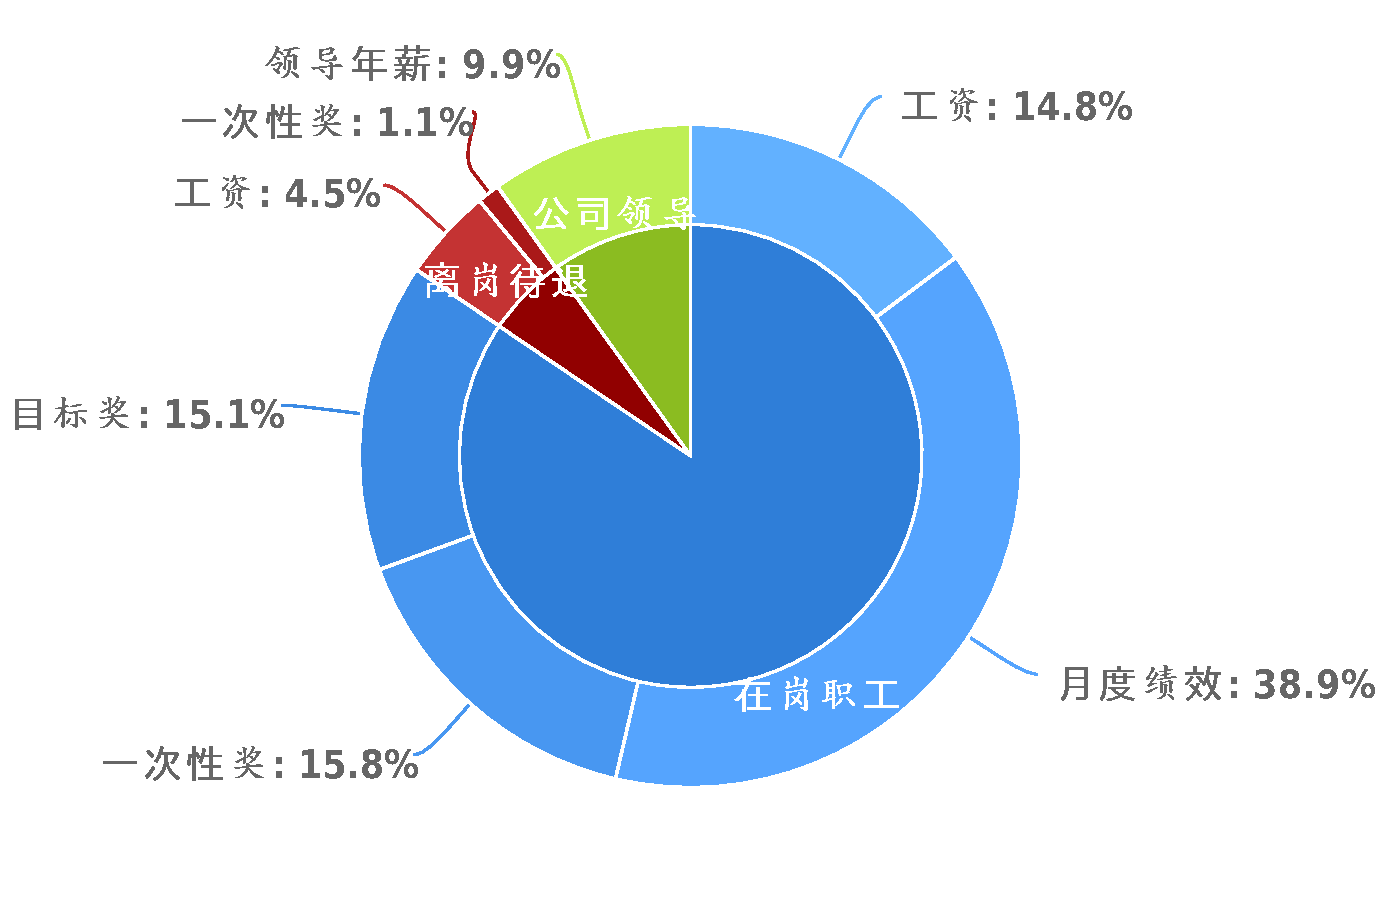
\includegraphics[width=0.8\textwidth]{fig2_1.pdf}
  \caption{2013年工资使用情况}
  \label{figure2-1}
\end{figure}
%%%%%%%%%%%%%%%%%%%%%%%===Fig2-1===%%%%%%%%%%%%%%%%%%


一、在岗职工薪酬部分,共计19329899.76元,其中工资使用3379641.28元,月度绩效使用8889646.56元,一次性奖使用3611559.92元,目标奖使用3449052元。

二、离岗待退职工薪酬部分,共计1282898.85元,其中工资使用1035683.06元,一次性奖使用247215.79元。

三、公司领导年薪使用2262200元。





%%%%%%%%%%%%%%%%%%%%%%%%%%%%%%%%%%%%%%%%%%%%%%%%%%%%%%%%%%%%%%%%%%%%%%%%%%%%%%%%%%%%%%%%%%%%%%%


\section{2013年接受审计的情况报告}

一、国家局派遣会计师事务所对公司2012年代财务决算报表进行审计。\textbf{审计结论:}审计报告未出具保留意见。


二、配合国家税务总局开展税收风险管理工作专项检查,对2008年-2012年度各税纳税情况进行全面自查和清理。\textbf{整改结果:}并于年内补交税款合计36276 元,其中增值税16829元、企业所得税6647元、印花税10919元、城建教育费附加2004元。

三、根据川渝中烟统一部署,对公司2010年至2012年各项审计中发现的问题开展审计整改工作。\textbf{整改结果:}大额现金使用问题,于2014年3月整改完成。职工宿舍一套权属不一致问题,因历史遗留原因尚未整改落实。


四、开展2012年预算执行和重点费用使用情况自查、2012年合同执行情况自查,并接受川渝公司审计部的复查。\textbf{复查结论:}抽查业务招待费、会议费未见异常;合同执行情况审计建议3条:建议今后加强立项和招投标过程的程序性管理。加强单一来源采购的程序管理。完善单一来源采购方式确定依据。针对以上建议,公司在2013年的过程控制中加以整改。


五、根据川渝公司要求,配合科达信会计师事务所,开展对原总经理韩勇同志的离任审计工作,经过15个工作日审计,目前已结束现场审计。\textbf{审计结论:}审计报告正在拟定中。


